\documentclass[a4paper,14pt]{extarticle}

\usepackage[utf8]{inputenc}
\usepackage[T2A]{fontenc}
\usepackage[english, russian]{babel}

\usepackage[mode=buildnew]{standalone}
\usepackage{setspace}


% Различные пакеты
\usepackage{
	amssymb, amsfonts, amsmath, amsthm, physics,
	cancel, indentfirst,makecell,multirow, 
	graphicx, tikz, mathtools, float, setspace,caption,subcaption
} 

\usepackage{mathtools}

% Эта опция включает нумерацию только у тех формул,
% на которые есть ссылка в документе
\mathtoolsset{showonlyrefs=true} 

 % Цвета для гиперссылок
\definecolor{linkcolor}{HTML}{000000} % цвет ссылок
\definecolor{urlcolor}{HTML}{799B03} % цвет гиперссылок
 
\usepackage{xcolor}
\usepackage[
    unicode, 
    colorlinks, 
    urlcolor=urlcolor, 
    linkcolor=linkcolor,
    citecolor=linkcolor
]{hyperref}

% Увеличенный межстрочный интервал, французские пробелы
\linespread{1.2} 
\frenchspacing 

%%%%%%%%%%%%%%%%%%%%%%%%%%%%%%
%  Пользовательские команды  %
%%%%%%%%%%%%%%%%%%%%%%%%%%%%%%


\makeatletter
    \newcommand{\fftStar}[1]{\mathfrak{F}^*\qty[#1]}
    \newcommand{\fftNoStar}[1]{\mathfrak{F}\qty[#1]}
    \newcommand{\fft}{
                 \@ifstar
                 \fftStar%
                 \fftNoStar%
    }
\makeatother

\makeatletter
    \newcommand{\ifftNoStar}[1]{\mathfrak{F}^{-1}\qty[#1]}
    \newcommand{\ifftStar}[1]{\qty(\mathfrak{F}^{-1}\qty[#1])^*}
    \newcommand{\ifft}{
                 \@ifstar
                 \ifftStar%
                 \ifftNoStar%
    }
\makeatother

\newcommand{\mean}[1]{\langle#1\rangle}
\newcommand\ct[1]{\text{\rmfamily\upshape #1}}
\newcommand*{\const}{\ct{const}}
\renewcommand{\phi}{\varphi}
\renewcommand{\epsilon}{\varepsilon}
%\renewcommand{\sigma}{\varsigma}


\captionsetup{subrefformat=parens}

\usepackage{array}
\usepackage{pstool}


% Диагональная ячейка в таблице ( типа |a/b|)
\newcolumntype{x}[1]{>{\centering\arraybackslash}p{#1}}
\newcommand\diag[4]{%
  \multicolumn{1}{p{#2}|}{\hskip-\tabcolsep
  $\vcenter{\begin{tikzpicture}[baseline=0,anchor=south west,inner sep=#1]
      \path[use as bounding box] (0,0) rectangle (#2+2\tabcolsep,\baselineskip);
      \node[minimum width={#2+2\tabcolsep},minimum height=\baselineskip+\extrarowheight] (box) {};
      \draw (box.north west) -- (box.south east);
      \draw (box.south west) -- (box.north west);
      \node[anchor=south west] at (box.south west) {\footnotesize#3};
      \node[anchor=north east] at (box.north east) {\footnotesize#4};
 \end{tikzpicture}}$\hskip-\tabcolsep}}

%%%%%%%%%%%%%%%%%%%%%%%%%%%%%
%  Геометрия и колонтитулы  %
%%%%%%%%%%%%%%%%%%%%%%%%%%%%%


\usepackage{geometry}
\geometry       
    {
        left            =   2cm,
        right           =   2cm,
        top             =   2.5cm,
        bottom          =   2.5cm,
        bindingoffset   =   0cm
    }

% Настройка содержания, точки после нумераций
\usepackage{tocloft}
\addto\captionsrussian{\renewcommand{\contentsname}{Оглавление}}
\renewcommand{\cftsecleader}{
	\cftdotfill{\cftdotsep}}
% \renewcommand{\thesection}{
	% \arabic{section}.}
% \renewcommand{\thesubsection}{
	% \arabic{section}.\arabic{subsection}.}
% \renewcommand{\thesubsubsection}{
	% \arabic{section}.\arabic{subsection}.\arabic{subsubsection}.}     
\usepackage[explicit]{titlesec}

% Колонтитулы
%\usepackage{fancyhdr} 
	%\pagestyle{plain} 
	%\fancyhead{} 
	%\fancyhead[R]{} 
	%\fancyhead[L]{} 
	%\fancyfoot{} 
	%\fancyfoot[C]{\thepage} 

\NewDocumentCommand{\codeword}{v}{%
\texttt{\textcolor{gray}{#1}}%
}
\usepackage{listings,multicol}
\usepackage{courier}
\definecolor{mygreen}{rgb}{0,0.6,0}
\definecolor{mygray}{rgb}{0.5,0.5,0.5}
\definecolor{mymauve}{rgb}{0.58,0,0.82}
\newcommand{\python}[1]{\lstinline[basicstyle=\normalsize\ttfamily]{#1}}

\lstset{ 
  backgroundcolor=\color{white},   % choose the background color; you must add \usepackage{color} or \usepackage{xcolor}; should come as last argument
  basicstyle=\footnotesize\ttfamily,        % the size of the fonts that are used for the code
  breakatwhitespace=false,         % sets if automatic breaks should only happen at whitespace
  breaklines=true,                 % sets automatic line breaking
  captionpos=b,                    % sets the caption-position to bottom
  commentstyle=\color{mygreen},    % comment style
  deletekeywords={...},            % if you want to delete keywords from the given language
  escapeinside={\%*}{*)},          % if you want to add LaTeX within your code
  extendedchars=true,              % lets you use non-ASCII characters; for 8-bits encodings only, does not work with UTF-8
  firstnumber=1,                % start line enumeration with line 1000
  frame=single,	                   % adds a frame around the code
  keepspaces=true,                 % keeps spaces in text, useful for keeping indentation of code (possibly needs columns=flexible)
  keywordstyle=\color{blue},       % keyword style
  language=Python,                 % the language of the code
  morekeywords={*,...},            % if you want to add more keywords to the set
  numbers=left,                    % where to put the line-numbers; possible values are (none, left, right)
  numbersep=15pt,                   % how far the line-numbers are from the code
  numberstyle=\tiny\color{mygray}, % the style that is used for the line-numbers
  rulecolor=\color{black},         % if not set, the frame-color may be changed on line-breaks within not-black text (e.g. comments (green here))
  showspaces=false,                % show spaces everywhere adding particular underscores; it overrides 'showstringspaces'
  showstringspaces=false,          % underline spaces within strings only
  showtabs=false,                  % show tabs within strings adding particular underscores
  stepnumber=1,                    % the step between two line-numbers. If it's 1, each line will be numbered
  stringstyle=\color{mymauve},     % string literal style
  tabsize=2,	                   % sets default tabsize to 2 spaces
  %title=\lstname,                   % show the filename of files included with \lstinputlisting; also try caption instead of title
  frame=none,
  %multicols=1,
  columns=fullflexible,
  extendedchars=\true,
  escapechar=!,
}




\title{Компьютерные технологии}
\author{Гвоздков Е.}



\begin{document}
\maketitle

\textbf{Задание 8} Постройте модель Солнечной системы. Рассчитайте параметры траектории кометы,
попавшей в Солнечную систему извне. Постройте зависимости скорости и координаты кометы
от времени при различных начальных параметрах, а также оцените точность интегрирования в
зависимости от схемы интегрирования и величины шага интегрирования.

\section{Описание модели Солнечной системы}
Для описания движения планет и кометы в поле тяготения Солнца примем несколько приближений:
\begin{enumerate}
	\item Планеты не влияют гравитацией друг на друга
	\item Описание движения будет происходить в плоскости, т.е. не учитывается координата $z$
	\item Комета не влияет на орбиты планет Солнечной системы
	\item Солнце неподвижно в начале координат
\end{enumerate}
Поскольку влиянием планет друг на друга принебрегается, их орбиты описываются определенным образом.
Траектория орбиты представляет из себя эллипс, в фокусе которого расположено тяготеющее тело, в данном случае Солнце.

\subsection{Описание движения планет}
Уравнение эллипса орбиты в полярных координатах задается следующим образом:
\begin{equation}
	r = \frac{a(1-e^2)}{1 + e \cos(\theta + \alpha)},
\end{equation}
где $a$ - большая полуось эллипса, $e$ - эксцентриситет, $\alpha$ - угловой сдвиг
эллипса относительно $\theta=0$.

Закон невозмущенного движения тела по эллиптической орбите из второго закона Кеплера имеет вид
\begin{equation}
	r^2\frac{d\theta}{d t} = \const = \sqrt{\mu a (1-e^2)},
\end{equation}
где $\mu = GM$ - гравитационный параметр ($G$ - гравитационная постоянная, $M$ - масса Солнца).

% Таким образом, для полного описания орбиты небесного тела необходимы следующие параметры
\begin{figure}[h!]
	\centering
	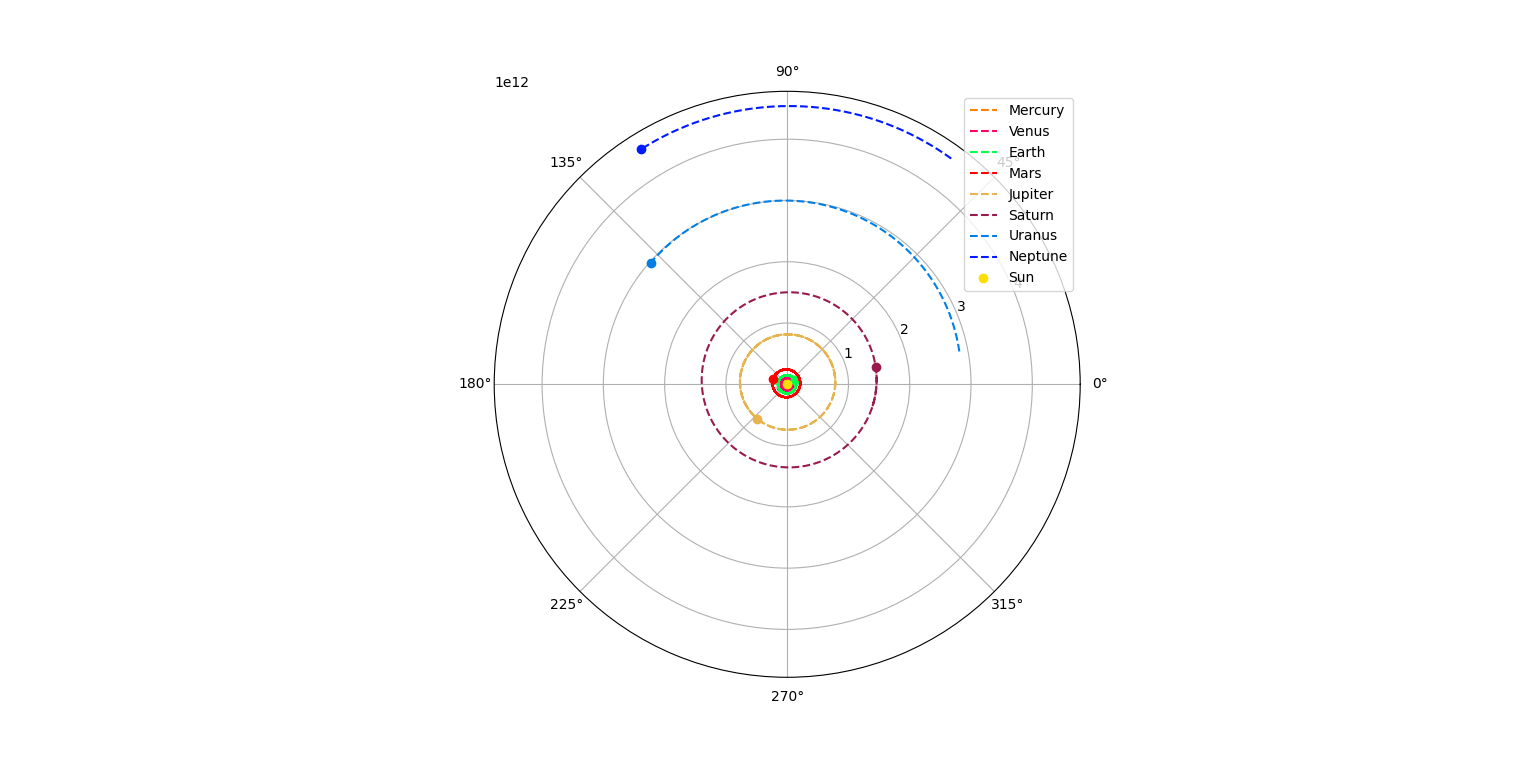
\includegraphics[width=0.8\linewidth]{imgs_8/solar.png}
	\caption{Модель Солнечной системы}
    \label{fig:system}
\end{figure}


\section{Описание движения кометы в Солнечной системе}
Движение тела в поле тяготения описываются законом всемирного тяготения
\begin{equation}
	F_g = G\frac{m_1 m_2}{R^2},
\end{equation}
где $m_1, m_2$ - массы тел, $R$ - расстояние между телами. Сила при этом направлена от кометы к планете.
В случае нескольких тел $N$, действующих
гравитацией на конкретное тело (комету), силы суммируются, и закон примет виде

\begin{equation}
	F_g = G m \sum_{i=0}^{N-1}\frac{m_i}{R_i^2},
\end{equation}
где $i$ - индекс, $m$ - масса кометы, $m_i$ - масса $i$-ой планеты, $R_i$ - расстояние между
кометой и $i$-той планетой.

Для моделирования влияния нескольких тел на движение кометы, воспользуемся вторым законом Ньютона:
\begin{equation}
	\vec{F} = m\vec{a} = \vec{F_g} = G m \sum_{i=0}^{N-1}\frac{m_i}{R_i^2}\vec{e_i},
\end{equation}
где $\vec{e_i}$ - единичный вектор, направленный от кометы к планете с индексом $i$.
Приведем выражение выше в другом виде
\begin{equation}
    \vec{r''} = G \sum_{i=0}^{N-1}m_i\frac{\vec{r_i}-\vec{r}}{R_i^3},
\end{equation}
где $\vec{r_i}$ - радиус вектор положения планеты с индексом $i$. Введем $\vec{v} = \vec{r'}$,
тогда получим следующую систему уравнений
\begin{equation}
	\vec{v'} = G \sum_{i=0}^{N-1}m_i\frac{\vec{r_i}-\vec{r}}{R_i^3}, \quad
	\vec{r'} = \vec{v}
\end{equation}

\section{Результаты моделирования}
Описание и моделирование системы производится на языке Python.
Начальными параметрами моделирования выступают первоначальные положения планет Солнечной системы,
а также начальные координаты и скорость кометы.

Планеты и их движение описываются классом $\codeword{CelestialBody}$ в файле $\codeword{SolarSystem.py}$.
Каждая планета - инстанция класса. Комета описывается отдельным классом $\codeword{Comet}$, в котором также 
присутствует метод \codeword{evaluate_model}, который является основным в моделировании.

\newpage
\section{Исходный код}
\lstinputlisting[label={lst:task8}, caption={Исходный код задания}]{SolarSystem.py}
\lstinputlisting[label={lst:task8_2}, caption={Исходный код задания}]{simulation.py}


\end{document}